\section{Experimental campaign on commodity CI}
\label{sec:exp}

\subsection{Setup and design}

The campaign runs in a public continuous-integration workflow on a four-core,
16~GB hosted runner. Constrained CI is the intended calibration setting:
accessible, reproducible, and usable when dedicated clusters are unavailable.
Each job provisions a Hyperledger Besu~\cite{besu} QBFT network of~$\n$
validators under the \RNM{} protocol (Definition~\ref{def:rnm}). A closed-loop
generator drives~$\cc$ concurrent submitters and records steady-state committed
throughput after warm-up. Faults are injected with kernel traffic control
(omission and duplication; not equivocation).

\textbf{X1}/\textbf{X3} calibrate $(\beta,\gamma)$ on a factorial grid;
\textbf{X2} checks the quota regime; \textbf{X3b} re-samples along
concurrency paths; \textbf{X4} varies emulated RTT; \textbf{X5} reports
detector rates; \textbf{X7}/\textbf{X8} check prediction-interval coverage and
sizing ablation. Cross-client replication (\textbf{X9}/GoQuorum) is out of
scope. In total $\resTotalRuns$ successful records,
$\approx\resCoreHours$ core-hours, $\n_{\max}=\resNmaxMeasured$.

\paragraph{Reproducibility.}
All experiments are reproducible from the public CI workflow and archived
artefacts at \url{https://github.com/bpenyak/Resource_Normalized_Scaling_Laws_for_Byzantine_Consensus}.

\subsection{Results}

\emph{X1/X3 --- bi-factor calibration.}
Joint OLS on the reference-quota subset yields
$\beta=\resBeta\pm\resBetaSE$ and $\gamma=\resGamma\pm\resGammaSE$
($R^{2}=\resRsq$; Table~\ref{tab:results}). Under \RNM{} one expects $\beta>0$
when concurrency is held fixed. The fit confirms that expectation at $\q=0.25$
within the evaluated deployment.

\emph{X3b --- path check of Proposition~\ref{prop:identifiability}.}
A single-factor fit along $\lambda=1$ gives $\ahat=\resAlphaHat$ against
$\gamma\lambda-\beta=\resAlphaPred$.
Figure~\ref{fig:confounding} shows measured exponents tracking
$\gamma\lambda-\beta$ within the investigated configuration --- consistency
with the analytical prediction, not universal validity of the bi-factor form.

\begin{figure}[!t]
\centering
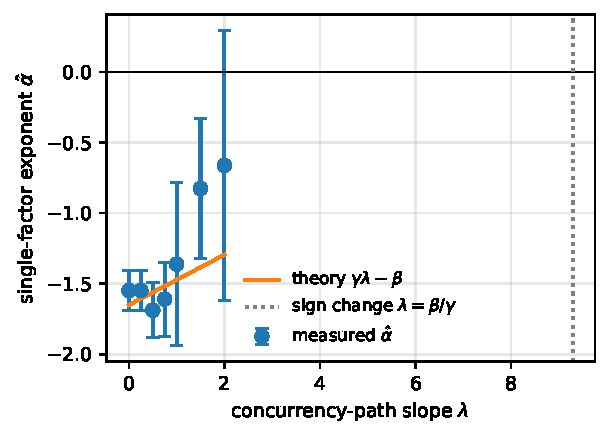
\includegraphics[width=0.36\textwidth]{figures/fig_confounding}
\caption{Measured $\ahat$ (points) vs.\ analytical $\gamma\lambda-\beta$
(line) in the evaluated deployment
(Proposition~\ref{prop:identifiability}).
Sign change at $\lambda=\beta/\gamma=\resLambda$}
\label{fig:confounding}
\end{figure}

\emph{X2 --- quota-regime check.}
The partial $F$-test for quota\,$\times\log\n$ interaction rejects pooling
across $\{0.20,0.25,0.33\}$ ($p=\resQinvP$): $\beta$ drops from
$\approx\resBetaQmid$ at $\q=0.25$ to $\resBetaQhigh$ at $\q=0.33$.
Deployment-specific coefficients are therefore reported at the reference quota
$\q=0.25$.

\emph{X4 --- latency.}
Under elevated emulated RTT, $\beta$ rises from $\resBetaRttZero$ to
$\resBetaRttHigh$ in this campaign. Calibration on LAN-like RTT is therefore
optimistic for geo-distributed deployments unless re-calibrated.

\emph{X5 --- detector.}
Omission/duplication detection yields AUC$\,=\,\resAuc$
(Figure~\ref{fig:roc}, near chance), so the workflow defaults to the
throughput-bound constraint under the evaluated detector.

\begin{table}[!t]
\centering
\caption{Calibrated parameters, quota check, detector, and coverage
(evaluated deployment)}
\label{tab:results}
\scriptsize
\begin{tabular}{lll}
\headline
Quantity & Estimate & Note \\
\headline
$\Tzero$; $\beta$; $\gamma$ &
  $\resTzero$; $\resBeta\pm\resBetaSE$; $\resGamma\pm\resGammaSE$ &
  bi-factor \\
$\csat$, $\theta$; $\hat\sigma$ & $\resCsat$, $\resTheta$; $\resSigmaRes$ &
  saturation / residual \\
$\ahat$ at $\lambda=0,1,2$ &
  $\resAlphaHatLzero$, $\resAlphaHatLone$, $\resAlphaHatLtwo$ &
  X3b \\
$\beta$ at $q=0.20,0.25,0.33$ &
  $\resBetaQlow$, $\resBetaQmid$, $\resBetaQhigh$ &
  X2, $p=\resQinvP$ \\
$\beta$ at RTT $0$/high & $\resBetaRttZero$, $\resBetaRttHigh$ & X4 \\
$\pd$, $\pf$, $\rho$; AUC &
  $\resPd$, $\resPf$, $\resRho$; $\resAuc$ &
  X5, $\thr=\resDetectorThr$ \\
coverage $90\%$/$95\%$ & $\resCovNinety$, $\resCovNinetyFive$ &
  hold-out $\resHoldoutN$ \\
\headline
\end{tabular}
\end{table}

\begin{figure}[!t]
\centering
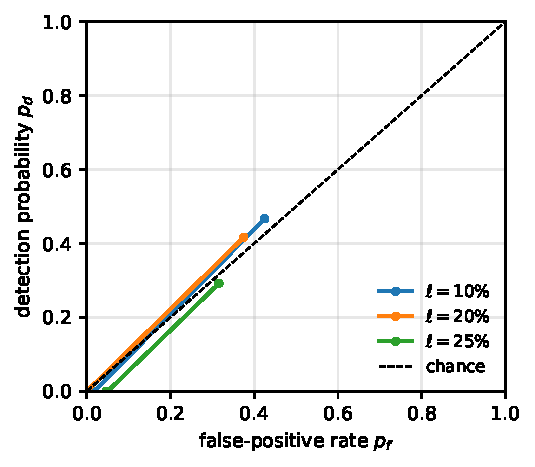
\includegraphics[width=0.34\textwidth]{figures/fig_roc}
\caption{Measured detector ROC (AUC$\,=\,\resAuc$, near chance); throughput
binds the window under the evaluated deployment}
\label{fig:roc}
\end{figure}

\emph{X7/X8 --- coverage, comparison, and ablation.}
Hold-out coverage meets the nominal levels in Table~\ref{tab:results} within
the calibrated range. The fitted covariance confirms that $\hat{V}$ is
nondecreasing for $\n\ge\resNmaxMeasured$, so~$h$ in~\eqref{eq:h} is strictly
decreasing on the model-based extrapolation range; on the measured grid we
evaluate~$h$ directly.
Out-of-sample log-RMSE for linear / single-factor / USL~\cite{gunther2007} /
bi-factor predictors is $\resRmseLinear$, $\resRmseSingle$, $\resRmseUsl$,
$\resRmseOurs$. The bi-factor improvement over USL is consistent with decoupling
concurrency from replica count under \RNM{}. Relative sizing costs:
$\resCostLinear$, $\resCostSingle$, $\resCostUsl$, $\resCostOurs$.
